\section{Software Tasks}
\label{cp4:corpus-tasks}

We start corpus creation by identifying software tasks 
for which a developer will likely benefit from 
the use of additional information to complete.
We scope task selection to \textit{Android development} 
because the 
Android \acf{SDK} evolves constantly due to 
functionality, security and performance-related improvements~\cite{Li2018android, Mateus2020}.
These improvements impact its development community, requiring them to often  seek information regarding changes in the SDK~\cite{linares2014, bavota2014b, mcdonnell2013}.
For example, over 35,000 developers have used Q\&A forums to discuss tasks covering 87\% of the classes in the Android API~\cite{parnin2012}.


Two common places where Android task can be found are:


\begin{itemize}
    \item the description of an issue
    (e.g., a bug or feature request) reported in an issue tracking system; or in
    \item a post in a community forum, development mailing lists, and others.
\end{itemize}

Several studies have used issue tracking system and software development communities for software tasks~\cite{Arya2019, baltes2019, nadi2020, Xu2017}
and, following the lead
of these studies, we select GitHub issues and \acf{SO} posts on Android development as 
the two sources for the tasks in our corpus.



\subsubsection{GitHub tasks}

To select tasks from GitHub, we are guided by studies that use 
stars~\cite{borges2016, borges2018}
as a proxy for a project's popularity~\cite{Ferreira2016, Xavier2020}.
We selected 14 projects,
ranging from mail clients\footnote{\url{https://github.com/k9mail/k-9}}
to development frameworks\footnote{\url{https://github.com/libgdx/libgdx}},
by filtering the list of top-starred projects in GitHub to those with the \textit{Java} and \textit{Android} tags.
We then randomly selected 25 distinct issues originating from these starred projects as the GitHub tasks of our corpus (average of 1.78 issues per project).
While selecting issues, we took care to check that they had at least one follow-up comment and that the issue title did not contain certain words, e.g., {\small \texttt{test}} or {\small  \texttt{ignore}},
as these words indicate issues  created automatically by scripts or bots---a common pitfall that researchers must be aware of when mining GitHub~\cite{kalliamvakou2014}.


Figure~\ref{fig:lock-screen-task} shows an example of a GitHub task in our corpus.
Although the expected behaviour is that the app controls should be visible even with the screen locked,  a user reports that the app screen is missing.
A developer addressing this issue might need to review the Android lock screen documentation~\cite{apiLockTask}
or refer to examples of applications that use the Android lock screen~\cite{mediumLockApp}.
For the remainder of this chapter, we use the lock screen task as a running example.


\begin{figure}
    \centering
    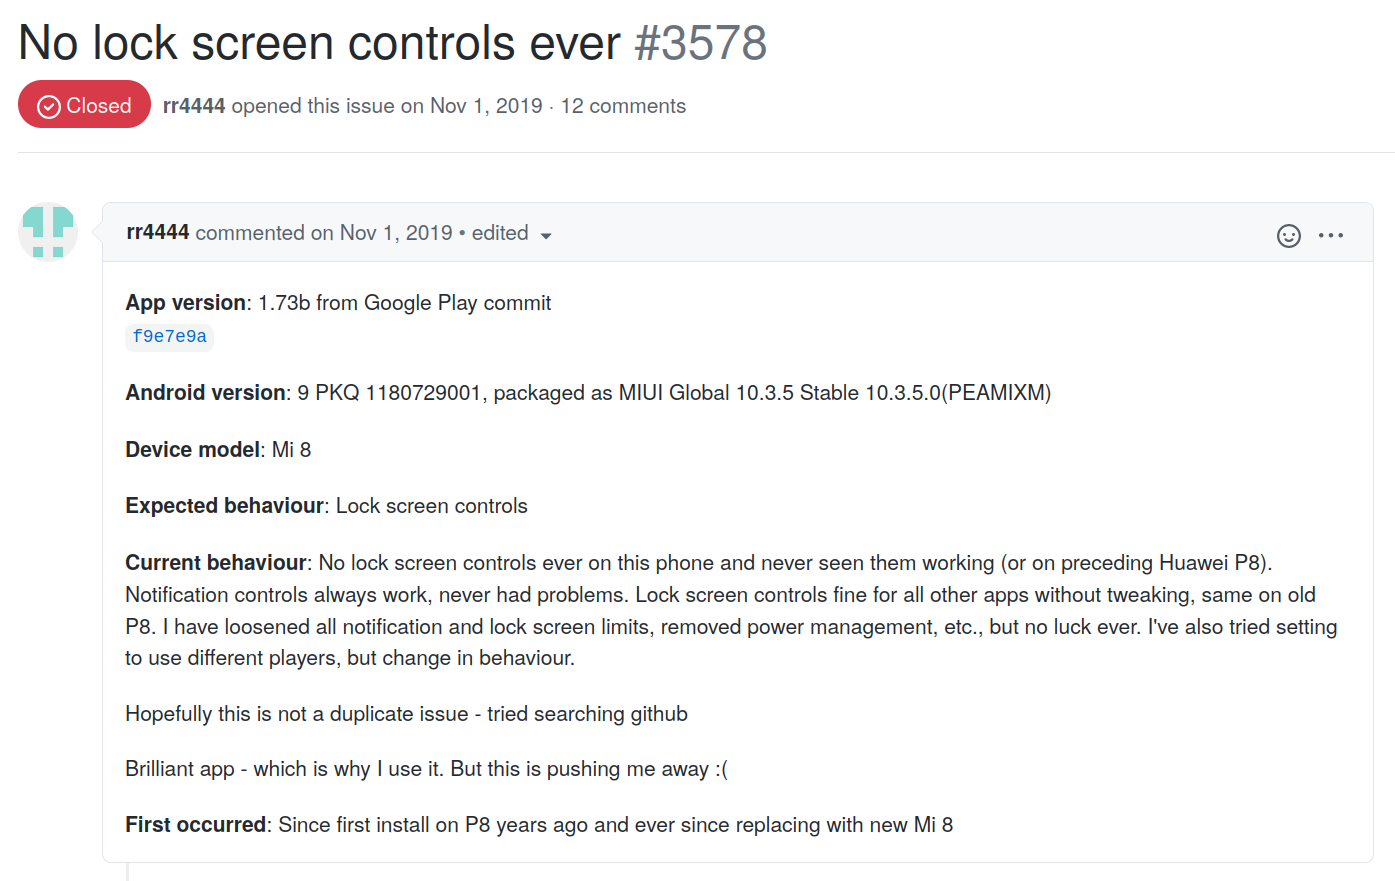
\includegraphics[width=\textwidth]{cp4/lock-screen-task}
    \caption{Sample GitHub task from our corpus}
    \label{fig:lock-screen-task}
\end{figure}



\subsubsection{Stack Overflow tasks}

%Provided that we restrict our corpus to tasks related to %the Android development domain,


We consider Stack Overflow posts as software tasks because to answer a post,
a developer often needs to provide references
supporting their answer~\cite{yazdaninia2021}.
Finding these references in a timely manner and writing the key information that helps a user understand 
 the provided solution encompasses many of the activities found in a developer's daily work, e.g., work-related browsing, coding, debugging, and reading/writing documentation~\cite{Meyer2017}.
For example, Figure~\ref{fig:webview-task} depicts a task where a developer describes her struggles using the Android WebView component~\cite{apiWebView}.
To answer this question, a developer will not only provide a code snippet, but also explain key points of the Android WebView API
and how they were used in the solution provided to the task, 
as presented in Figure~\ref{fig:webview-task-answer}.


\begin{figure}
    \centering
    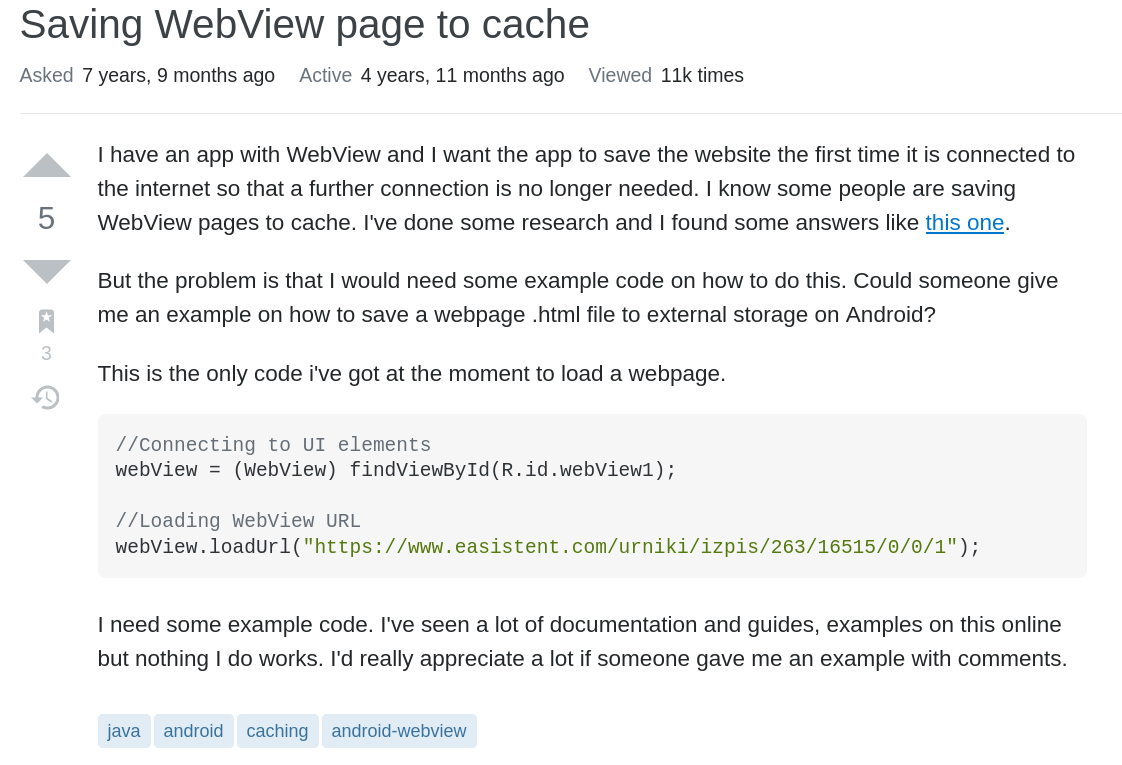
\includegraphics[width=0.85\textwidth]{cp4/webview-task}
    \caption{Sample Stack Overflow question}
    \label{fig:webview-task}
\end{figure}



\begin{figure}
    \centering
    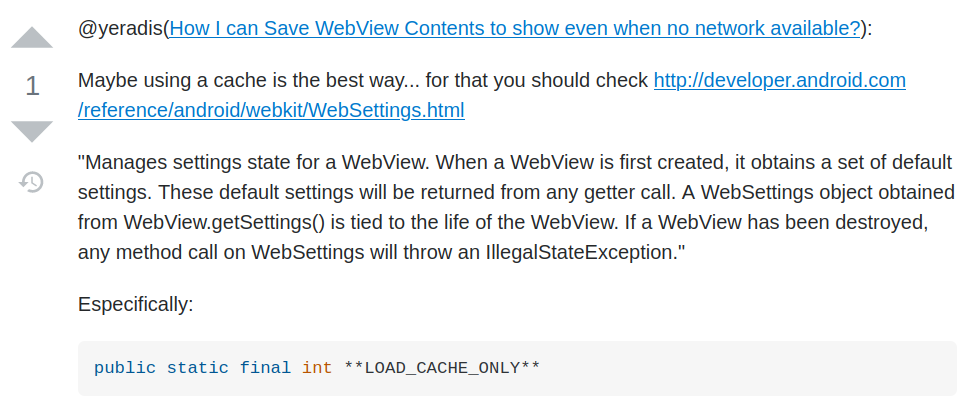
\includegraphics[width=0.85\textwidth]{cp4/webview-task-answer}
    \caption{Excerpt of a Stack Overflow answer}
    \label{fig:webview-task-answer}
\end{figure}

We randomly select 25 Stack Overflow posts from a curated list about Android development~\cite{baltes2020}.
This list was built by Baltes et al. 
using the Stack Overflow dump published on June 5, 2018~\cite{baltes2019-rep, SOTorrent2019}
and it contains 209,536 unique posts with the \textit{Java} and \textit{Android} tags.



% When selecting tasks in GitHub and Stack Overflow, a major challenge arises due to the sheer amount of data available.
% Baltes et al.~\cite{baltes2019} argues that even a cursory inspection of a sample set
% of Stack Overflow posts shows clear differences in a post's content or structure due to aspects such as programming languages, frameworks, associated technologies, and others.
% \gm{-It feels like there is a missing sentence about how differences relate
% to the 'sheer amount of data' and why the differences matter.}

% To ensure the tasks in the corpus we produce
% circumvent \gm{-circumvent has a negative connotation - is there a way
% to say this positively?} the heterogeneity of data on GitHub and Stack Overflow, we scope task selection to the \textit{Android} development domain. This decision
% restricts task selection to a single programming language (\textit{Java})
% while still enabling investigation of a domain that has been
% widely discussed by practitioners and researchers alike.
